\documentclass[a4paper,10pt]{article}
%\usepackage[latin1]{inputenc} % Paquetes de idioma (otro encoding)
\usepackage[utf8]{inputenc} % Paquetes de idioma
\usepackage[spanish]{babel} % Paquetes de idioma
\usepackage{graphicx} % Paquete para ingresar gráficos
\usepackage{grffile}
\usepackage{hyperref}
\usepackage{fancybox}
\usepackage{amsmath}
\usepackage{amsfonts}
\usepackage{listings}
\usepackage{pdfpages}
\usepackage{float}
\usepackage{bm}
\usepackage[font={footnotesize}]{caption}
\usepackage[labelformat=empty]{caption}
% Paquetes de macros de Circuitos
%\usepackage{pstricks}
% \usepackage{tikz}

% Encabezado y Pié de página
% Paquete para encabezados y pie de página
\usepackage{fancyhdr} 
% Sin esta línea no se imprimiría el encabezado en todas las páginas
\pagestyle{fancy} 

% Borra el encabezado anterior (Por defecto escribe el título de la 
%  sección en la que se encuentra la hoja
\fancyhf{} 
\setlength{\headheight}{22.55pt}
\fancyhead[L]{
	{\textsf{Facultad de Ingeniería $-$ Universidad de Buenos Aires 
    \\ 75.99 - Trabajo Profesional}}
}
%\addtocounter{page}{5}
\fancyhead[R]{\thepage}

% Ajusta el tamaño de las líneas separadoras en el pié de página
\renewcommand{\footrulewidth}{0.4pt}
 % Ajusta el tamaño de las líneas separadoras en el encabezado
\renewcommand{\headrulewidth}{0.4pt} 

\fancyfoot[L]{
	{\textsf{Propuesta de Trabajo Profesional} \\
	{\textsf{Integrantes: Torres Feyuk, Germano Zbrun, Lopez Skuba}}
	}
}
		

% Carátula del Trabajo
\title{ \author{} % Lo pongo para que el warning no moleste :p
\setlength{\unitlength}{1cm} %  Especifica la unidad de trabajo
\thispagestyle{empty}

\begin{picture}(18,0)
\put(0,0){
\includegraphics[width=1.5cm, height=3cm]{Imagenes/Logo1.png}}

\put(10.5,0){
\includegraphics[width=3cm, height=3cm]{Imagenes/Logo2.png}}

\end{picture}
\\[1.5cm]
\begin{center}
	\textbf{{\Huge Facultad de Ingeniería \\ Universidad de Buenos Aires}}
    \\[1cm]
	{75.99 - Trabajo Profesional}\\[0.5cm]
    {MLC version 3 (Machine Learning Control)}\\[1.5cm]
\end{center}

\begin{flushleft}
	\textbf{Tutor: Adriana Echeverría} \\
    \textbf{Co-Tutor: Julia Garibaldi} \\[1cm]
	\textbf{Integrantes:} \\[1cm]

	\begin{tabular}{|c|c|c|}
		\hline
		\textbf{\normalsize Padrón} & \textbf{\normalsize Nombre}
                                    & \textbf{\normalsize Email} \\
		\hline
		\normalsize 89579 & \normalsize Torres Feyuk, Nicolás R. Ezequiel
                          & \normalsize ezequiel.torresfeyuk@gmail.com \\
		\hline
		\normalsize 86882 & \normalsize Germano Zbrun, Marco
                          & \normalsize marco.germano@intraway.com \\
		\hline
		\normalsize 88430 & \normalsize Lopez Skuba, Raúl
                          & \normalsize raullopez0@gmail.com \\
		\hline
	\end{tabular}
\end{flushleft}
\date{} % Hace que no se imprima la fecha en la cual se compilo el .tex
 }

\begin{document}
	\maketitle % Hace que el título anterior sea el principal del documento
	\newpage

    % Esta línea genera un indice a partir de las secciones y
    % subsecciones creadas en el documento
	\tableofcontents
	\newpage

    \section{Introducción Teórica} \label{sec:intro}
        El presente trabajo se propone el análisis, diseño e implementación de un conjunto de mejoras requeridas por Thomas Duriéz,
        investigador del laboratorio de fluidodinámica de la facultad de ingeniería, a aplicarse sobre el sistema MLC, desarrollado por él,
        y utilizado como herramienta en su trabajo de investigación. El siguiente capítulo fue realizado basado en la información obtenida
        en \cite{Duriez2016}.

        \subsection{Control a Lazo Cerrado optimizado a través de Función de Costo} \label{sec:close_loop}
        La teoría de control clásica categoriza los sistemas de control en \textbf{Open-Loop Control Systems} y
        \textbf{Close-Loop Control Systems} \cite{Ogata2002}. Se definen los mismos a continuación:

        \begin{itemize}
            \item \textbf{Open-Loop Control Systems:} Son aquellos sistemas en donde la salida del sistema no es comparada contra una
            referencia de entrada. Estos sistemas funcionan a base de calibración. Ejemplos de los mismos puede son pavas eléctricas,
            balanzas, etc.. Un esquema de este modelo es mostrado en la figura \ref{fig001}.
            \item \textbf{Closed-Loop Control Systems:} También llamados sistemas retroalimentados (Feedback Control Systems). Esta clase
            de sistema compara la salida retroalimentada contra una referencia de entrada, obteniendo así una función de error. La señal
            retroalimentada (feedback signal) puede ser la salida del sistema o bien una función derivada de la misma. La función de error
            es utilizada para especificar la actuación a ingresar en el sistema físico. Ejemplos de los mismos son el sistema de frenos
            ABS o la termorregulación corporal, entre otros. Un esque de este modelo es mostrado en la figura \ref{fig002}.
        \end{itemize}

        \begin{figure}[!Hhtb]
            \centering
            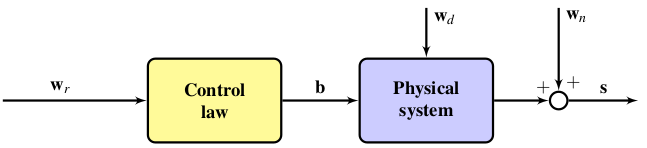
\includegraphics[width=12cm,origin=c]{Imagenes/open_loop.png}
            \caption{\textbf{Fig. 1} Open-Loop Control System, siendo $\mathbf{w_r}$ la señal de referencia, \textbf{b} la señal de
            actuación, $\mathbf{w_d}$ perturbaciones externas, $\mathbf{w_n}$ ruido introducido por los sensores involucrados y
            \textbf{s} la señal de salida} \label{fig001}
        \end{figure}

        \begin{figure}[!Hhtb]
            \centering
            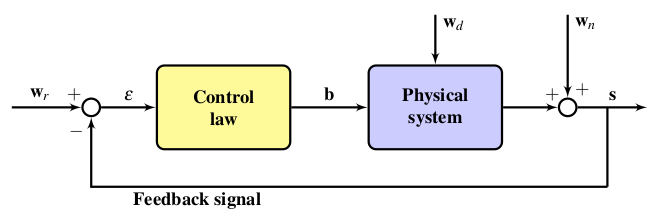
\includegraphics[width=12cm,origin=c]{Imagenes/closed_loop.png}
            \caption{\textbf{Fig. 2} Closed-Loop Control System, siendo $\mathbf{w_r}$ la señal de referencia, \textbf{b} la señal
            de actuación, $\bm{\varepsilon}$ la función de error, $\mathbf{w_r}$ perturbaciones externas, wn ruido introducido por los
            sensores involucrados y \textbf{s} la señal de salida} \label{fig002}
        \end{figure}

        Si bien los sistemas de control a lazo cerrado son complejos de diseñar y mantener, son los únicos que permiten estabilizar
        aquellos sistemas físicos que se ven afectados por estímulos externos. Esto último no es posible de realizar en un sistema de
        lazo abierto. Es por esta razón que este tipo de modelo es el mayormente usado para resolver problemas de naturaleza compleja
        (no lineales, caóticos, etc.) con un alto grado de interacción con variables externas.
        \indent Diseñar la ley de control que logre estabilizar el sistema deseado es un reto. Esto se debe a que, además de tener una
        comprensión matemática del sistema físico, se deben tener en cuenta todas las variables externas que modifican al mismo. Por esta
        razón, es importante tener una medida de la calidad de la ley de control propuesta. En la figura \label{fig003} se muestra un
        sistema a lazo cerrado con la adición de una función de costo \textbf{J}. Esta función de costo es la clave para lograr definir
        luego un método efectivo para encontrar leyes de control a través del MLC.

        \begin{figure}[!Hhtb]
            \centering
            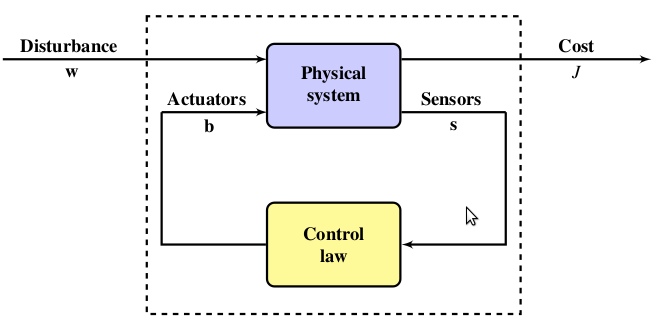
\includegraphics[width=12cm,origin=c]{Imagenes/control_loop.png}
            \caption{\textbf{Fig. 3} Sistema de Control a Lazo Cerrado de Costo \textbf{J}} \label{fig003}
        \end{figure}

        \subsection{Motivación} \label{sec:motiv}
        La estabilización de flujos turbulentos es una de las ramas más estudiadas dentro del control de fluídos. Las
        dificultades presentes en la resolución de este tipo de problemas, sumado a la gran cantidad de campos de aplicación, hacen del
        mismo un tema atractivo para científicos alrededor del mundo. Se listan a continuación algunas de las características más
        importantes:

        \begin{itemize}
            \item La cantidad de grados de libertad (debido a la naturaleza no lineal y caótica de los mismos) \textbf{dificulta la
            modelización del sistema físico}
            \item La naturaleza no lineal de esta clase de flujos impide aplicar el principio de superposición sobre los efectos producidos
            por cada actuador.
            \item Perturbaciones externas como el \textit{frequency crosstalk} \textbf{impiden encontrar una ley de control que lleve a la
            convergencia del sistema}, aún cuando se haya realizado una correcta modelización del mismo.
            \item Los flujos turbulentos poseen \textbf{estabilidad estacionaria} (existen valores definidos para variables estadísticas
            como la media y varianza). Esto permite que el sistema vuelva a su estado original luego de ser estimulado, haciendo posible
            la reproducibilidad de los experimentos a realizar.
        \end{itemize}

        Teniendo en cuenta las características enumeradas, el campo de los fluídos turbulentos permite encontrar leyes de control válidas
        basadas en prueba y error. Esto fue lo que motivó el desarrolló del framework MLC, el cual se describe a continuación.

    \subsection{MLC} \label{sec:mlc}
    \subsubsection{Arquitectura}
        MLC es un framework utilizado para descubrir leyes de control. Tiene como fin generar modelos de sistemas de forma automática,
        los cuales llamaremos controladores, a través de información de la calidad de la solución generada. Esta información es procesada
        a través de métodos basado en \textit{Machine Learning}, los cuales están diseñados para buscar nuevos controladores dentro del
        espacio de soluciones existente. La arquitectura básica del mismo se exhibe en la figura \ref{fig004}.

        \begin{figure}[!Hhtb]
            \centering
            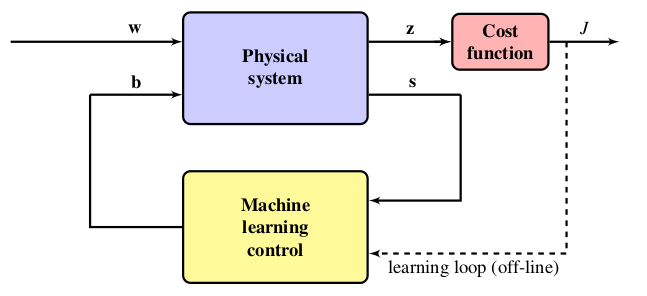
\includegraphics[width=12cm,origin=c]{Imagenes/MLC_architecture.png}
            \caption{\textbf{Fig. 4} Arquitectura del MLC} \label{fig004}
        \end{figure}

        \indent Comparando las figuras \ref{fig003} y \ref{fig004}, se puede observar como la ley de control es reemplazada por el MLC,
        el cual recibe como entrada los valores sensados \textbf{s} y el valor \textbf{J}, resultante de la aplicación de la función de
        costo ante la salida del sistema físico excitado. En función de estas muestras, MLC genera una nueva ley de control la cual es
        evaluada, obteniendo un nuevo valor de \textbf{J}.

    \subsubsection{Machine Learning y Programación Genética} \label{sec:mlc_and_gp}
        \textbf{Machine Learning} es una subrama de las ciencias de la computación basada en las campos de \textit{Pattern Recognition} y
        \textit{Computational Learning Theory}. La misma es utilizada, entre otros usos, para identificar sistemas dentro de un espacio de
        soluciones de alta dimensionalidad (\textit{high dimensional search space}) a través de técnicas de aprendizaje. Existe una gran
        cantidad de técnicas a utilizar dentro del campo de \textbf{Machine Learning}, tales como \textit{Gradient Search} o
        \textit{Monte-Carlo Statistical Analysis}, pero las mismas poseen como característica principal la obtención de soluciones
        subóptimas o asociadas con un costo alto cuando el espacio de soluciones es extremadamente grande \cite{Duriez2016}. Es aquí
        donde entran en juego los algoritmos
        evolucionarios, los cuales han demostrado ser óptimos a la hora de resolver este tipo de problemas. \\

        \indent La \textit{Programación Genética} y los \textit{Algoritmos Genéticos} se basan en la propagación de generaciones de
        individuos, llamadas poblaciones, los cuales son seleccionados en función del valor de su \textit{fitness}. Cada individuo tiene
        asociado un \textit{costo} o \textit{fitness} el cual es obtenido luego de evaluar el mismo a través de una función de costo.
        Un individuo en este ámbito \textit{tiene una correspondencia directa con la estructura y parámetros que definen
        a una ley de control}. En la figura \ref{fig005} se exhibe un diagrama detallado del uso de estos algoritmos dentro de la solución
        implementada en MLC. Un individuo $\mathbf{b = K(s)}$ es evaluado en el sistema dinámico. De dicha evaluación, se obtiene su
        \textit{fitness} \textbf{J}. Al terminar de evaluar una población entera, MLC genera una nueva población a través del uso de
        diferentes técnicas de \textit{Programación Genética}. Este proceso se exhibe en detalle en la sección \ref{sec:law_gen}.

        \begin{figure}[!Hhtb]
            \centering
            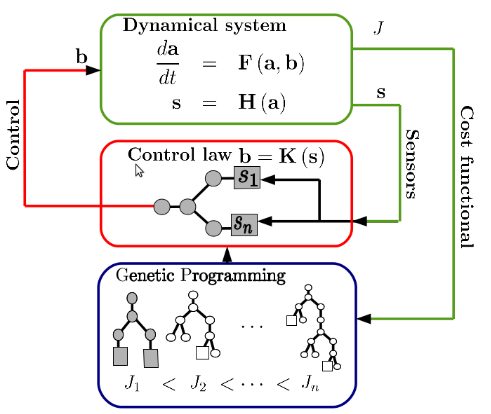
\includegraphics[width=9cm,origin=c]{Imagenes/MLC_block_diagram.png}
            \caption{\textbf{Fig. 5} Generación de nuevas leyes de control} \label{fig005}
        \end{figure}

        Un individuo se encuentra modelizado dentro del MLC como un conjunto de funciones y parámetros que poseen la forma de un
        \textit{recursive function tree}. Las funciones matemáticas utilizadas son las operaciones +, -, $\times$, / con el agregado
        de cualquier otro tipo de función, como puede llegar a ser un coseno, una exponencial o una tangente hiperbólica por nombrar
        algunas. Los nodos hojas poseen constantes o bien parámetros del sistema (por lo general sensores), mientras que los nodos no hoja
        poseen las funciones matemáticas anteriormente nombradas. La figura \ref{fig006} muestra la modelización de un individuo.
        La composición de los individuos a través de \textit{trees} hacen de los mismos candidatos ideales para ser utilizados como input
        dentro de \textit{algoritmos genéticos}.

        \begin{figure}[!Hhtb]
            \centering
            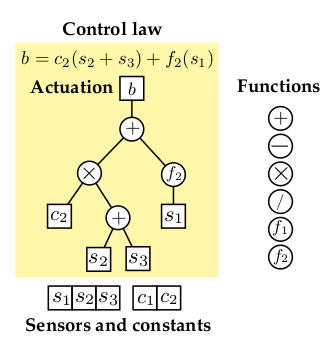
\includegraphics[width=6cm,origin=c]{Imagenes/individual_tree.png}
            \caption{\textbf{Fig. 6} Individuo $\mathbf{b = K(s_1, s_2, s_3)}$ visto como un \textit{recursive funcion tree}
            } \label{fig006}
        \end{figure}


    \subsubsection{Generación de nuevas Leyes de Control} \label{sec:law_gen}
        \indent La primera población de individuos es generada de forma aleatoria en función de los sensores, constantes y funciones
        matemáticas a disposición y la misma no posee un costo asociado a priori. La población luego es evaluada (el proceso de evaluación
        es explicado en la sección \ref{sec:mlc_gp}), con lo cual se obtiene el \textit{fitness} asociado a cada individuo. A partir de
        este punto se procede a evolucionar la población. Dicha evolución se lleva a cabo a través de los siguientes algoritmos
        \cite{Duriez2016}:

        \begin{itemize}
            \item \textbf{Elitismo:} Se eligen a los mejores individuos de la población evaluada y se agregan directamente en la próxima
            generación.
            \item \textbf{Replicación:} De forma aleatoria, se eligen algunos individuos de la población evaluada y se hace avanzar a los
            mismos a la próxima población.
        \item \textbf{Crossover:} Se toman a dos individuos que posean un \textit{fitness} similar y se intercambian de forma aleatoria
            algunas ramas del \textit{recursive tree} asociado a cada uno.
            \item \textbf{Mutación:} Se modifican de forma aleatoria los parámetros o funciones de ciertos individuos.
        \end{itemize}

        Luego de realizar la evolución de la población se procede nuevamente a evaluar a la misma. A partir de este momento, ese proceso
        se repite hasta que se llega a algún punto de corte. Por lo general, el punto de corte del algoritmo utilizado por MLC consiste
        en la cantidad de generaciones evaluadas y evolucionadas hasta el momento. Otro punto de corte que se puede utilizar es haber
        alcanzado algún \textit{fitness} deseado en el mejor individuo. En la figura \ref{fig007} se muestra un diagrama de flujo
        explicando el proceso de generación de nuevas poblaciones.

        \begin{figure}[!Hhtb]
            \centering
            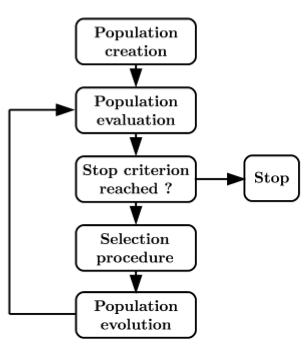
\includegraphics[width=6cm,origin=c]{Imagenes/flow_diagram.png}
            \caption{\textbf{Fig. 7} Diagrama de Flujo del proceso de Generación de Poblaciones} \label{fig007}
        \end{figure}


    \newpage
    \section{Objetivo}
        Durante los años que Thomas ha estado trabajando en el sistema MLC se ha encontrado con una serie de dificultades técnicas y
        funcionales. Durante el segundo cuatrimestre del 2015, como parte de un trabajo práctico de la asignatura 75.61 Taller de
        Programación III, se trabajó sobre el sistema MLC, relevando los requerimientos e implementando en forma parcial alguno de ellos.
        Los mismos se listan a continuación:

        \begin{itemize}
            \item Migrar el sistema de MATLAB a Python.
            \item Generar un set de pruebas unitarias, de integración y funcionales.
            \item Refactorizar el código existente de manera de lograr un diseño más flexible y extensible que el actual.
            Se espera que la nueva solución sea capaz de abarcar una mayor cantidad de problemas sin necesidad que el usuario deba
            modificar en forma sustancial el código del programa.
            \item Analizar los cuellos de botella presentes en la versión actual del programa. Los tiempos de uso del laboratorio son
            acotados por lo tanto se espera que la nueva implementación mejore esos tiempos permitiendo ejecutar una mayor cantidad de
            pruebas.
            \item Implementar una interfaz gráfica para la configuración del sistema y el análisis de los resultados.
        \end{itemize}

    \newpage
    \section{Alcance}
    \subsection{Requerimientos Funcionales}
        \begin{itemize}
            \item Migrar el sistema completo de matlab a python. Esto incluye la implementación del algoritmo genético y la comunicación
            con el sistema de control.
            \item Diseñar e implementar un modelo de persistencia de la aplicación basado en base de datos.
            \item Re-diseñar e implementar el sistema de control (componente que se ejecuta sobre la plataforma Arduino). Se debe analizar
            la implementación actual del componente. Las mejoras deben enfocarse principalmente en la performance del componente.
            \item Diseñar e implementar un protocolo de comunicación que permita configurar el sistema de control, enviar los individuos de
            la población, correr el algoritmo y obtener los resultados desde el programa principal.
            \item Desarrollar una API genérica que permita comunicar al sistema MLC con el sistema embebido. De esta forma se busca
            desacoplar al sistema en su totalidad de algún dispositivo de hardware específico, dejando abierta la posibilidad de poder
            cambiar el mismo por alguna otra plaqueta (Raspberry, beagleboard, etc.) en un futuro.
            \item Implementar una interfaz gráfica que permita configurar los parámetros de entrada del sistema.
            \item Implementar una interfaz gráfica para la visualización y el análisis de los resultados de las corridas.
        \end{itemize}

    \subsection{Requerimientos No Funcionales}
        \begin{itemize}
            \item El sistema debe ser multiplataforma y debe estar implementado con tecnologías de software libre.
            \item Definir un conjunto de métricas de calidad a aplicarse a lo largo del proyecto.
            \item Generar un set de pruebas de integración que permitan validar el funcionamiento del sistema con el cliente.
            \item Implementar un conjunto de test unitarios que garanticen la cobertura de código de los módulos del sistema de acuerdo
            a las métricas de calidad definidas.
            \item Relevar qué métricas se están usando en el laboratorio para medir la performance y qué números está manejando Thomas en
            este momento.
            \item Realizar un estudio de mercado sobre las tecnologías embebidas comerciales existentes, de forma de encontrar el producto
            óptimo que cumpla con la relación velocidad de comunicación / precio.
        \end{itemize}

    \section{Hardware}
    \subsection{MLC}
        MLC no posee limitaciones de hardware conocidas. Por esta razón, se toma como mínimo hardware requerido para ejecutar la
        aplicación el mínimo requerido por un sistema Unix. Los requerimientos mínimos se listan a continuación:

        \begin{itemize}
            \item Procesador x86 de 1 GHZ
            \item 512 MB RAM (1 GB recomendado)
            \item 20 GB de espacio en disco (la mayoría de este espacio está destinado a la instalación del MATLAB. En un futuro cuando
            se remueva la dependencia con MATLAB podrá reducirse este número)
        \end{itemize}

    \subsection{Sistema de Control}
        Los dispositivos utilizados para realizar el sensado de magnitudes físicas y la actuación de dispositivos físicos son Arduinos.
        El modelo utilizado del mismo por el momento no se sabe con exactitud, pero se están realizando con el modelo Due.

    \section{Software}
        En su versión terminada, el sistema correrá enteramente en Python 2.7. Durante la migración, se deberá utilizar MATLAB en una
        versión superior a la R2014B debido al módulo Python Engine requerido para poder establecer una comunicación entre ambos lenguajes
        de programación. La base de datos a utilizar será SQLite, debido a la simplicidad de los datos a almacenar y lo fácil, flexible y
        ligero que resulta este motor de BD embebido.

    \newpage
    \section{Metodología}

    \newpage
    \section{Cronograma}

    \newpage
    \bibliography{mybib}{}
    \bibliographystyle{ieeetr}

\end{document}

